\markboth{GUI tools}{GUI tools}
\section{GUI tools}
\label{sec:GUI}
For a quick and easy set-up of a battery model, two GUI tools were created as part of this package. Since both tools are based on \java\ Swing, a \java\ virtual machine (JVM) must be installed for the GUI tools to function. Normally, \matlab\ comes pre-bundled with a JVM. However, in the rare cases in which this is not the case, an error message is printed to the command window.

\subsection{Battery Pack Designer}
\label{sec:designer}
The Battery Pack Designer is a GUI that enables the creation of a \mcode{batteryPack} object. It can be started by typing
\begin{lstlisting}
batteryPack.GUI
\end{lstlisting}
into the command window. Figure~\ref{fig:Designer} shows a screenshot of the tool in Windows. Usage of the tool should be self-explanatory. Detailed information is provided using tool tips, which appear when hovering over GUI element (i.e. button or text field) with the mouse. When the model is fully configured, a \mcode{batteryPack} object can be created and sent to the workspace. The Battery Pack Designer provides a comfortable way to create models for users who are new to the package. It can be practicable for the purpose of getting to know the model and it's interface. \\
However, it is not recommended to save the created objects in MAT files for later use in simulations. Object links within the model (i.e. the link between the age model and the pack; see section~\ref{sec:ageModel}) are broken upon saving, which may result in unexpected behaviour of the loaded objects. 
\begin{figure}[b!]
	\captionsetup{type=figure}
	\centering
	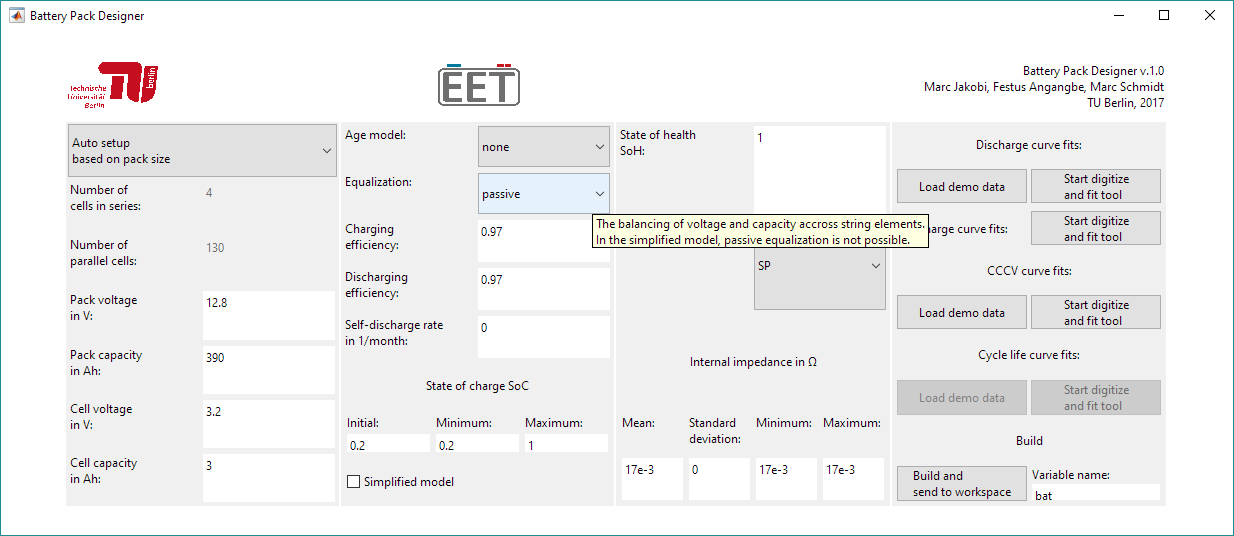
\includegraphics[width=\textwidth]{Designer.png}
	\caption[Screenshot of the Battery Pack Designer in Windows]{Screenshot of the Battery Pack Designer in Windows.}
	\label{fig:Designer}
\end{figure}
Furthermore, if multiple battery cells hold references to a single \mcode{dischargeCurves} object (see section~\ref{sec:dischargeCurvesMain}), the object is deep-copied across all of the cells, potentially resulting in large amounts of data\footnote{This can be fixed by re-adding the \mcode{dischargeCurves} using the \mcode{addcurves()} method after loading.}. The creation of deep-copies upon saving could also lead to memory leaks. Due to this behaviour, it is recommended to initialize the \mcode{batteryPack} at runtime, before the simulation (see section~\ref{sec:batteryPackConstructor}).\\
The Battery Pack Designer contains demo curve fits that can be loaded into the model. Alternatively, user-defined curves can be digitized and fitted using the provided digitizer and curve fit tool, which can be loaded from the Battery Pack Designer or from the command window.

\subsection{Digitizer and curve fit tool}
\label{sec:digitizeTool}
In order to use the created \mcode{batteryPack} object in a simulation, curve fits are required. Attempting to call the object's methods without having added at least a discharge curve will result in an error (see sections~\ref{sec:dischargeCurves} and~\ref{sec:batteryPack}). The digitizer and curve fit tool is provided in this pack for the purpose of digitizing bitmap images from data sheets and optionally pre-fitting the curves. It can be used for creating discharge curve fits (\mcode{dischargeCurves} objects), cycle life curve fits (\mcode{woehlerFit} objects), CCCV charging curve fits (\mcode{cccvFit} objects) and for extracting data from any other type of curve that can be used for later curve fitting.
\begin{figure}[b!]
	\captionsetup{type=figure}
	\centering
	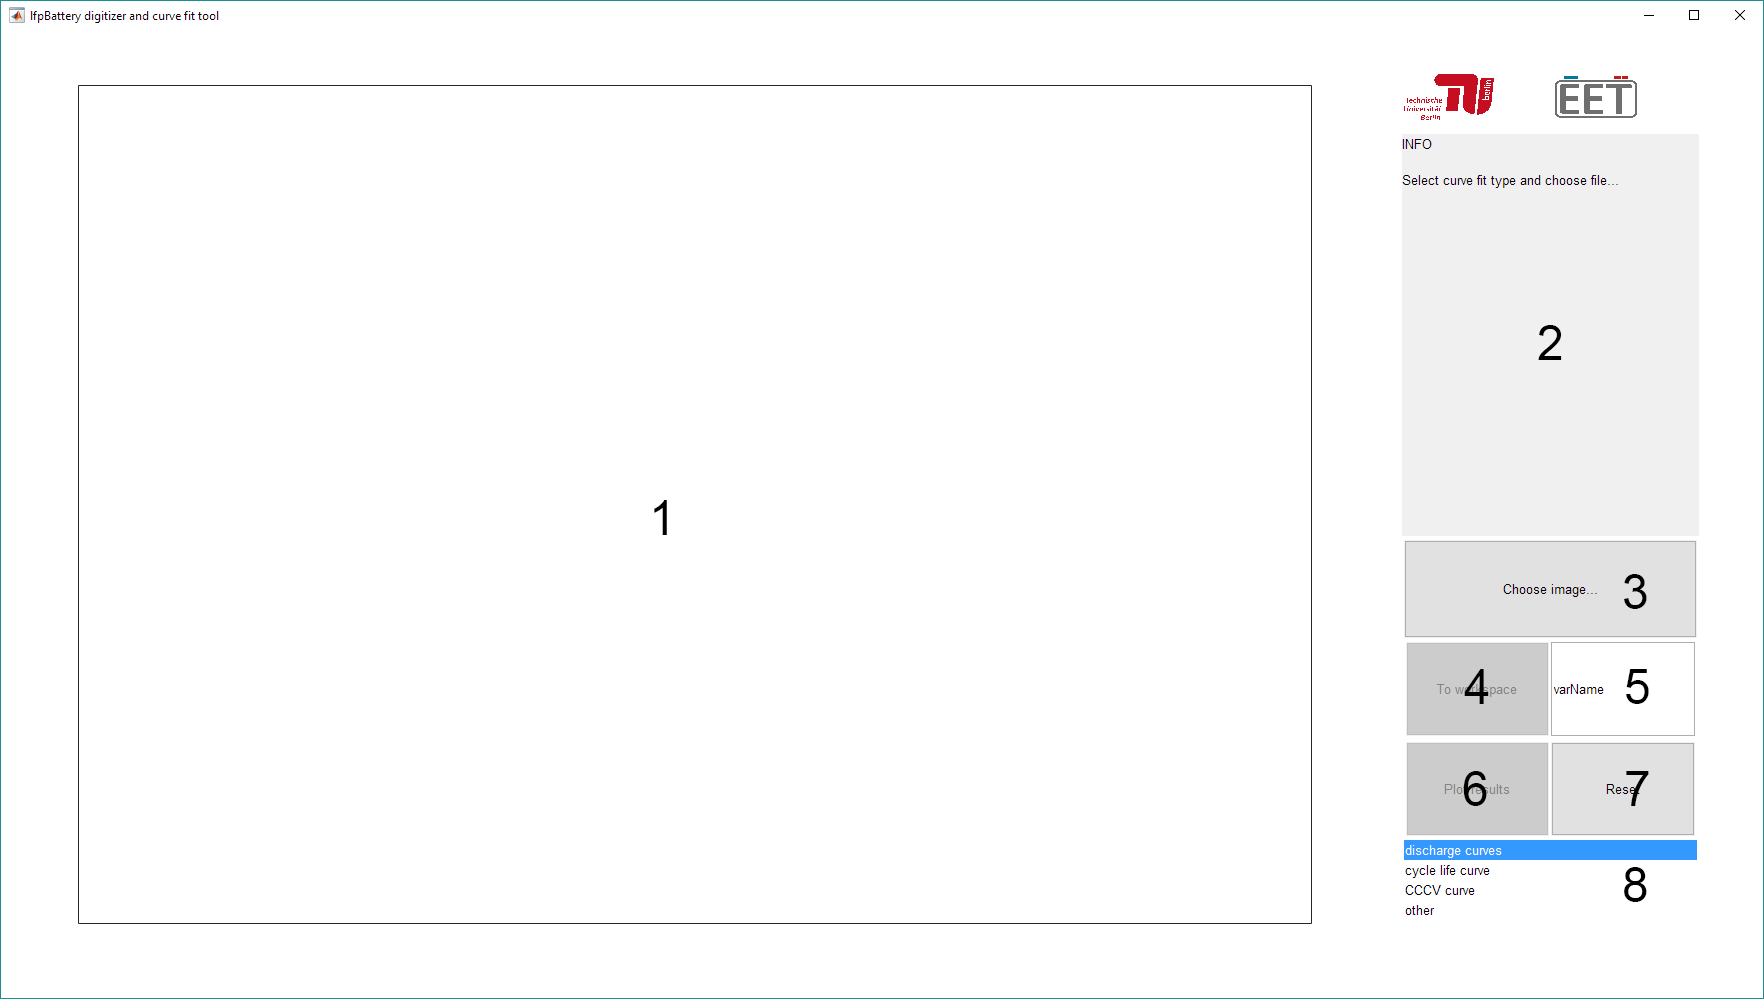
\includegraphics[width=\textwidth]{digitizeTool01.png}
	\caption[Screenshot of the digitizer and curve fit tool in Windows]{Screenshot of the digitizer and curve fit tool in Windows.}
	\label{fig:digitizeTool01}
\end{figure}
The tool can by started by typing
\begin{lstlisting}
batteryPack.digitizeTool
\end{lstlisting}
into the command window. Variations of it can also be started from the Battery Pack Designer. A screenshot of the tool after starting it is displayed in Figure~\ref{fig:digitizeTool01}. The components (numbered from 1 to 8) are described in the following:
\begin{enumerate}
	\item Axes in which the image that the data is extracted from is displayed.
	\item Information box that contains instructions for the current step (walkthrough).
	\item Opens a file chooser for loading the image of the curve that is to be digitized. Any bitmap format that can be displayed with the \mcode{imread()} function is accepted.
	\item Sends a Struct that contains the raw data and curve fit(s) to the workspace.
	\item Name of the Struct that is sent to the workspace.
	\item Plots the results of the curve fit against a scatter of the raw data.
	\item Resets the tool to it's initial state for fitting of a new curve.
	\item Selector for the type of curve. Changing the selection puts the tool in a state with code that is optimized for the selected curve type. Selecting "other" disables curve fitting and enables the digitizing of any 2-dimensional data set from an image.
\end{enumerate}
Before starting the digitization process, a bitmap image of the curve is required. For example, the Windows Snipping Tool can be used to extract the image from a PDF data sheet and save it as a PNG file. To load the file into the tool, click on the "Choose image..." button. This will open a file chooser that contains a preview pane. If the selected image can be previewed by the file chooser, the image can be digitized (see Figure~\ref{fig:file_chooser}).
\begin{figure}[b!]
	\captionsetup{type=figure}
	\centering
	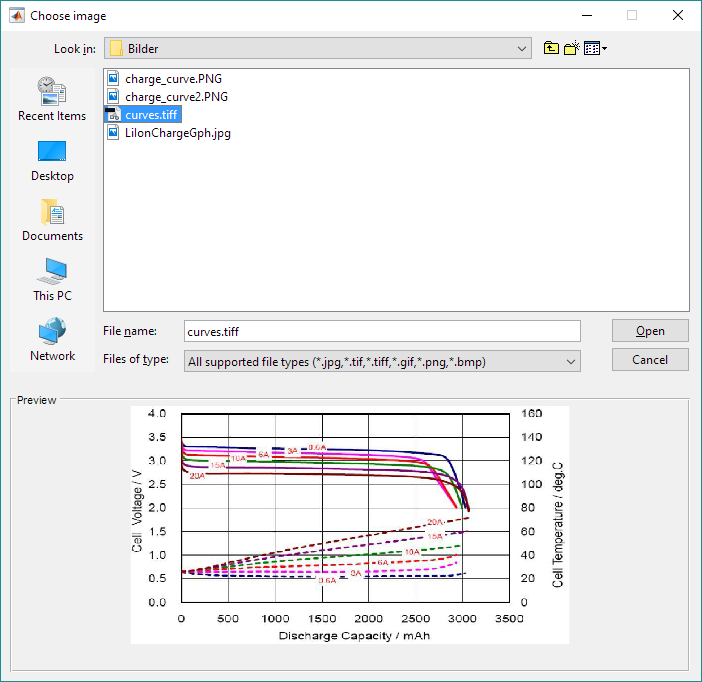
\includegraphics[width=.57\textwidth]{file_chooser.png}
	\caption[Screenshot of the \mcode{digitizeTool}'s file chooser with a preview pane]{Screenshot of the \mcode{digitizeTool}'s file chooser with a preview pane.}
	\label{fig:file_chooser}
\end{figure}
\begin{figure}[t!]
	\captionsetup{type=figure}
	\centering
	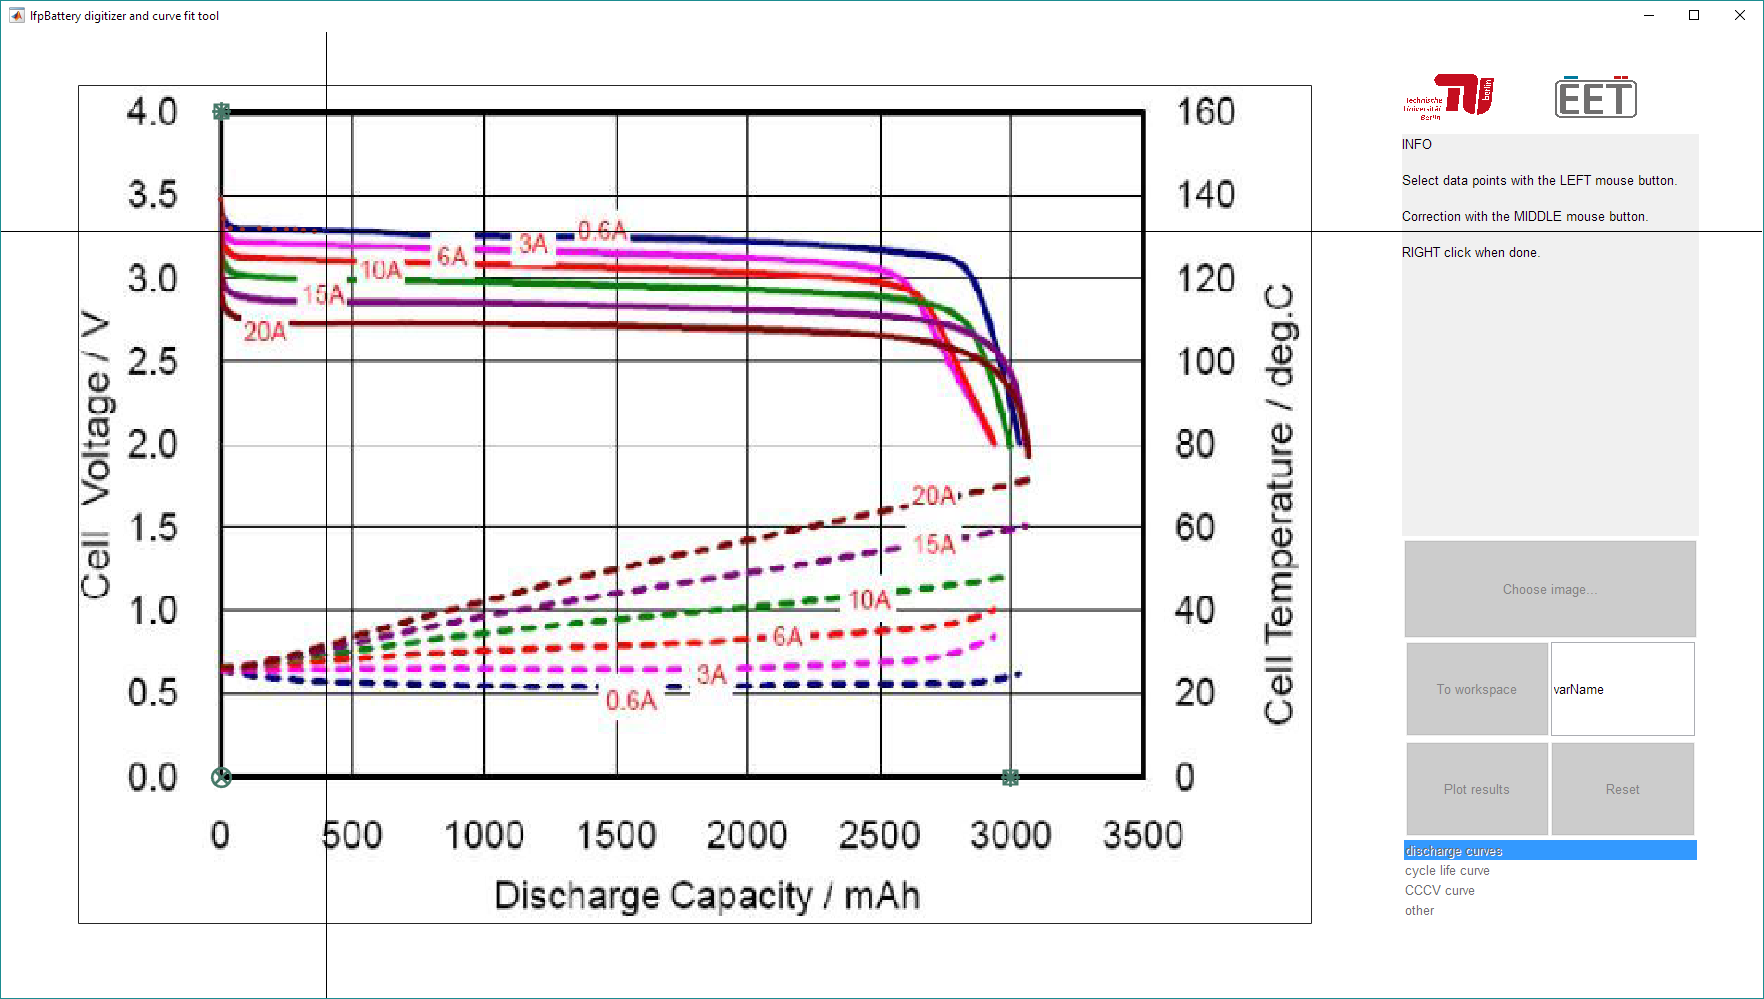
\includegraphics[width=\textwidth]{digitizeTool02.png}
	\caption[Screenshot of an image being digitized]{Screenshot of an image being digitized. The curves were extracted from~\cite{_data_2010}.}
	\label{fig:digitizeTool02}
\end{figure}
Once a file is selected the image is loaded into the axes window and the user is walked through the steps of defining the origin, x and y axis scales and number of data sets, etc. When everything is defined, the data can be selected using a mouse (see Figure~\ref{fig:digitizeTool02}). A mouse with 3 buttons (left, right, middle/scroll wheel) is recommended, so that corrections of poorly selected data can be performed.